
%----SECTION----
% \newpage
\section{Experiments}


%----SECTION----
\subsection{Settings}
We evaluate DVP-VAE on dynamically binarized MNIST \citep{lecun1998mnist} and OMNIGLOT \citep{lake2015human}. Furthermore, we conduct experiments on natural images using the CIFAR10 dataset \citep{alex2009learning}. We provide all the hyperparameters for training DVP-VAE in Appendix \ref{appendix:hyperparams} and in the code repository\footnote{\url{github.com/AKuzina/dvp_vae}}.
%----SECTION----
\subsection{Main Quantitative and Qualitative Results}\label{sect:exp_image_generations}

 \begin{table}[t]
        \centering
        \caption{The test performance: negative log likelihood on MNIST and OMNIGLOT, and bits-per-dimension (BPD) on CIFAR10.\\
        \textsuperscript{$\ddagger$} Results with data augmentation.\\
        \textsuperscript{$*$} Results averaged over 4 random seeds. Standard deviation reported in parentheses. 
        }
        \label{tab:main_results}
        \small{
        \begin{tabular}{l||lll|lll}
            \toprule
            \multirow{2}{*}{\textsc{Model}} & \multirow{2}{*}{\small{\textsc{L}}} & \footnotesize{\textsc{MNIST}} & \footnotesize{\textsc{OMNIGLOT}} & \multicolumn{3}{c}{\footnotesize{\textsc{CIFAR10}}}\\ 
                & &  \multicolumn{2}{c|}{$ - \log p(\rvx) \leq \, \downarrow $} & \small{\textsc{Size}} & \small{\textsc{L}} & \small{\textsc{bpd $ \leq \, \downarrow $}}\\
            \midrule
            \textbf{DVP-VAE} \normalsize{(ours)} & 8 
                    & \textbf{77.10}$^*$\footnotesize{(0.05)} & \textbf{89.07}$^*$\footnotesize{(0.10)}  
                    & 20M & 28 & \textbf{2.73}\\
            Attentive VAE \small{\citep{apostolopoulou2021deep}}  & \multirow{1}{*}{15}
                    & \multirow{1}{*}{77.63} & \multirow{1}{*}{89.50} & 119M & 16 & 2.79\\
            CR-NVAE \small{\citep{sinha2021consistency}}               & \multirow{1}{*}{15}
                    & \multirow{1}{*}{76.93\textsuperscript{$\ddagger$}} & \multirow{1}{*}{---} & 131M & 30 & 2.51\textsuperscript{$\ddagger$} \\
            VDVAE \small{\citep{Child2020-ze}} & --- & --- & --- & 39M & 45& 2.87 \\
            OU-VAE \small{\citep{pervez21a}} & \multirow{1}{*}{5}
                    & \multirow{1}{*}{81.10} & \multirow{1}{*}{96.08}         
                    & 10M & 3 & 3.39 \\
                    % \small{\citep{pervez21a}} \\
            NVAE \small{\citep{vahdat2020nvae}}& \multirow{1}{*}{15}
                    & \multirow{1}{*}{78.01} & \multirow{1}{*}{---} 
                    & --- & 30 & 2.91 \\
            BIVA\small{\citep{maaloe2019biva}}   & 6
                    & 78.41 & 91.34 & 103M & 15 & 3.08 \\
            VampPrior \small{\citep{tomczak2018vae}} & \multirow{1}{*}{2}
                    & \multirow{1}{*}{78.45}  &   \multirow{1}{*}{89.76}             
                    & --- & --- & --- \\
            LVAE \small{\citep{sonderby2016ladder}} & \multirow{1}{*}{5}
                    & \multirow{1}{*}{81.74} & \multirow{1}{*}{102.11}     
                    & --- & --- & --- \\
            IAF-VAE\small{\citep{kingma2016improved}} & \multirow{1}{*}{---}
                    & \multirow{1}{*}{79.10}  &   \multirow{1}{*}{---}             
                    & --- & 12 & 3.11 \\
            % \midrule
            % & \multicolumn{6}{c}{\footnotesize{Diffusion models}}\\
            % Improved DDPM \citep{nichol2021improved} &  --- & --- & --- &  & & 2.94 \\
            % VDM \citep{kingma2021variational} &  --- & --- & --- &  & & 2.64\\
            % DiffEnc \citep{nielsendiffenc} &  --- & --- & --- &  & & 2.62\\
            % NDM \citep{bartosh2023neural}&  --- & --- & --- &  & & 2.70\\
            \bottomrule
        \end{tabular}% % \end{varwidth}%\hfill 
        }
 \end{table} 
We report all results in Table \ref{tab:main_results}, where we compare the proposed approach with other hierarchical VAEs. 
We observe that DVP-VAE outperforms most of the VAE models\footnote{CR-NVAE \citep{sinha2021consistency} uses NVAE model and considerably improves its performance by applying data augmentations. We did not use any augmentations to compare fairly with all other hierarchical VAEs and were able to get a better NLL than NVAE and more recent hierarchical VAE models.
} while using fewer parameters than other models. For instance, on CIFAR10, our DVP-VAE requires 20M weights to beat Attentive VAE with about 6 times more weights.
Furthermore, because of the smaller model size, we were able to obtain all the results using a single GPU. 
We show the unconditional samples in Figure~\ref{fig:dct_samples} (see Appendix~\ref{appendix:samples} for more samples). 
The top row of each image shows samples from the diffusion-based VampPrior (i.e., pseudoinputs), while the second row shows corresponding samples from the VAE. 
We observe that, as expected, pseudoinputs define the general appearance of an image, while a lot of details are added later by the TopDown decoder. 
This effect can be further observed in Figure~\ref{fig:generative_recon} where we plot the reconstructions using different numbers of latent variables. In the first row, only a pseudoinput corresponding to the original image is used (i.e., $\rvu \sim r(\rvu|\rvx)$) while the remaining latent variables are sampled from the prior with low temperature. Each row below uses more latent variables from the variational posterior grouped by the scales. 
Namely, the second row uses the pseudoinput above and all the $4\times4$ latent variables from the variational posterior, then the third row uses additionally $8\times8$ latent variables, and so on. 

 \begin{figure}[t]
    \begin{tabular}{c}
        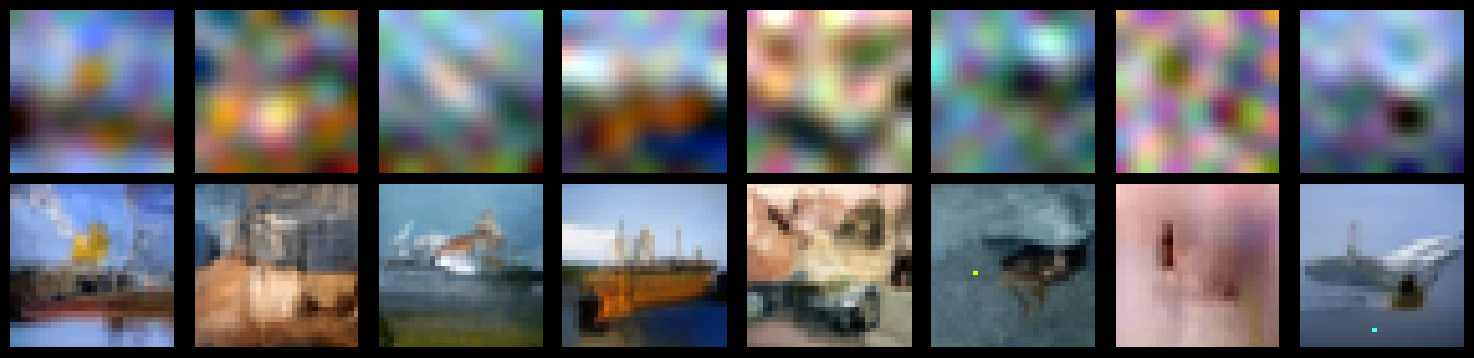
\includegraphics[width=0.85\textwidth]{pics/5_dvp/cifar10_dct_prior_samples.pdf} \\
        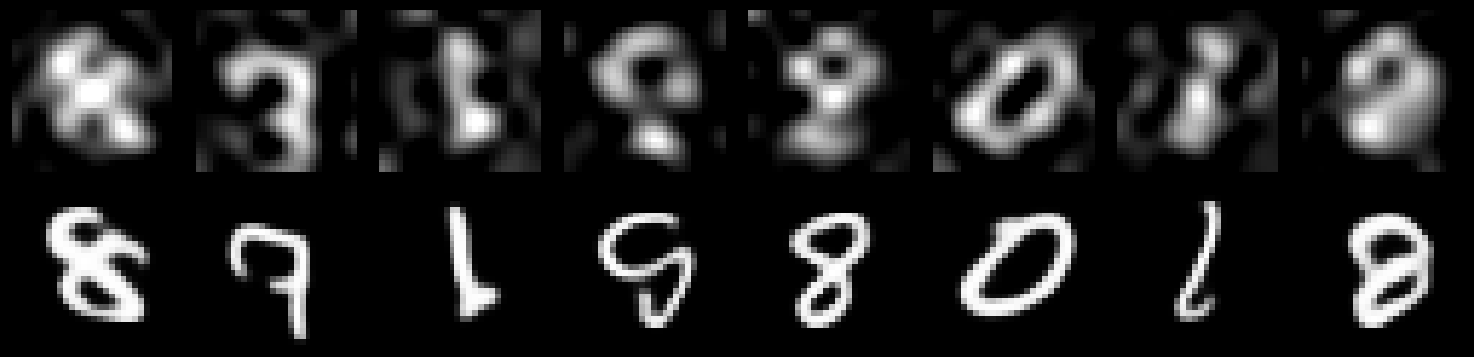
\includegraphics[width=0.85\textwidth]{pics/5_dvp/mnist_dct_prior_samples.pdf} \\
        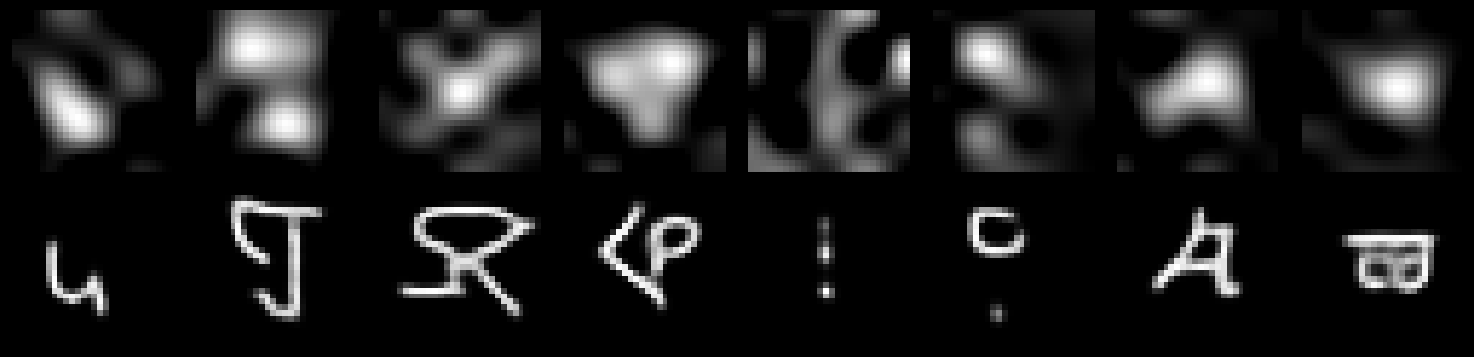
\includegraphics[width=0.85\textwidth]{pics/5_dvp/omniglot_dct_prior_samples.pdf} \\
    \end{tabular}
    \caption{Unconditional samples from the Diffusion-based VampPrior (top) and corresponding samples from the DVP-VAE (bottom).}
    \vskip -5pt
    \label{fig:dct_samples}
\end{figure}

\begin{figure}[t]
    \begin{tabular}{cc}
        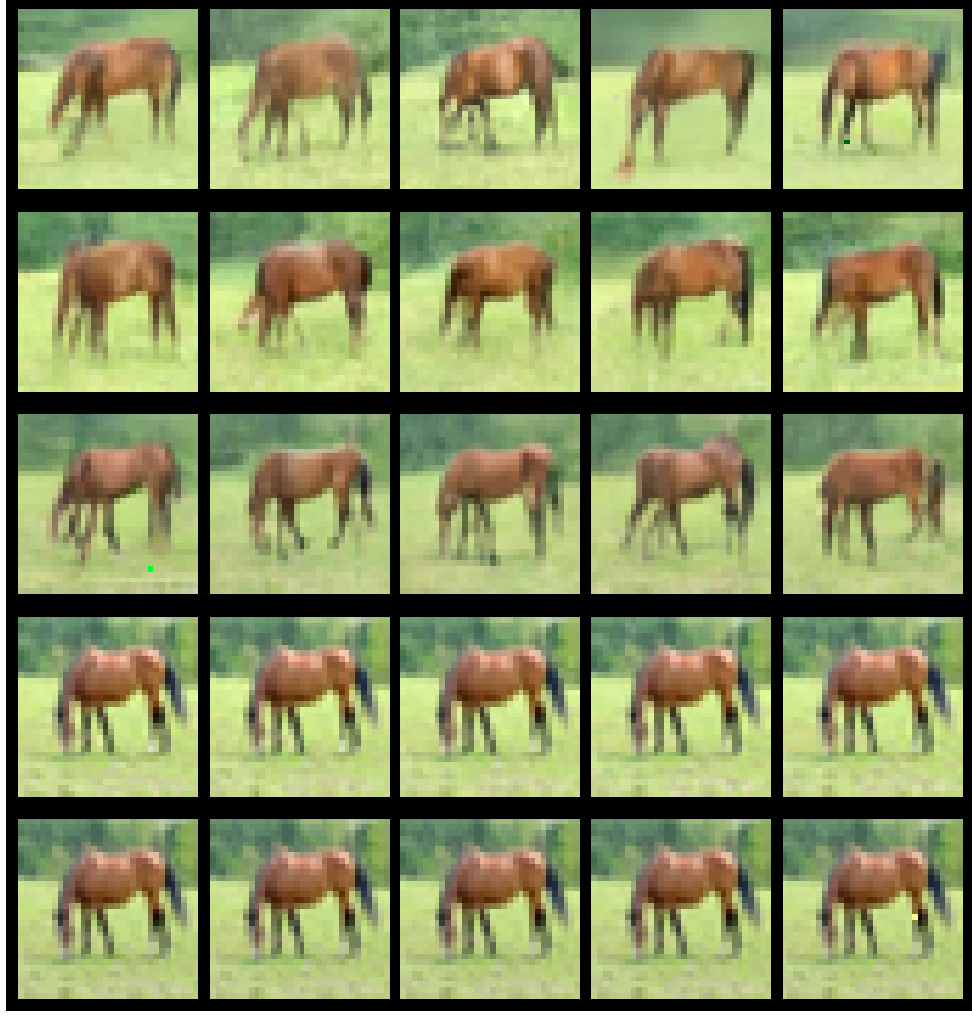
\includegraphics[width=0.43\textwidth]{pics/5_dvp/cifar10_generative_rec_6.pdf} &
        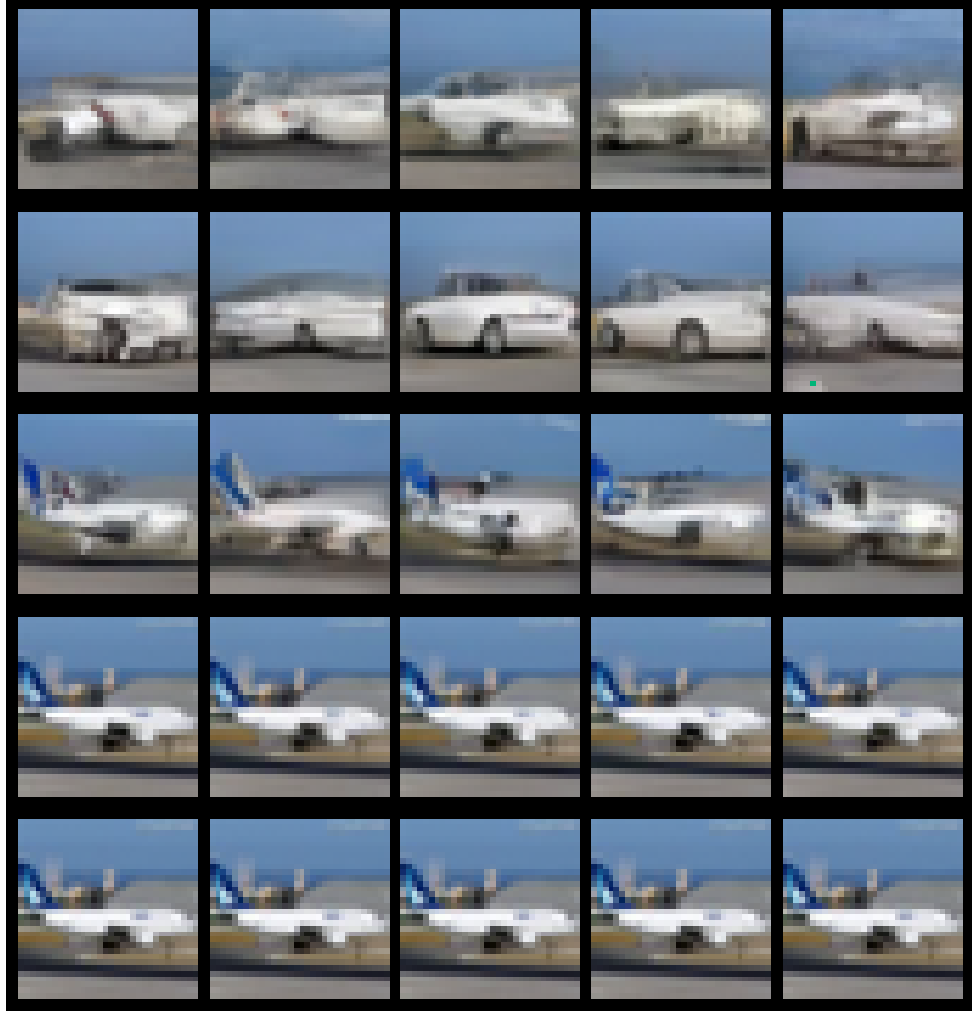
\includegraphics[width=0.43\textwidth]{pics/5_dvp/cifar10_generative_rec_9.pdf} \\ 
    \end{tabular}
    \caption{\textit{Generative reconstruction}s. The top row is using a pseudoinput sampled from $r(\rvu|\rvx)$ \textbf{only}.}
    \vskip -5pt
    \label{fig:generative_recon}
\end{figure}
% \begin{table}[t]
% \begin{minipage}[t]{0.45\linewidth}
% \begin{figure}[H]
%     \begin{tabular}{c}
%         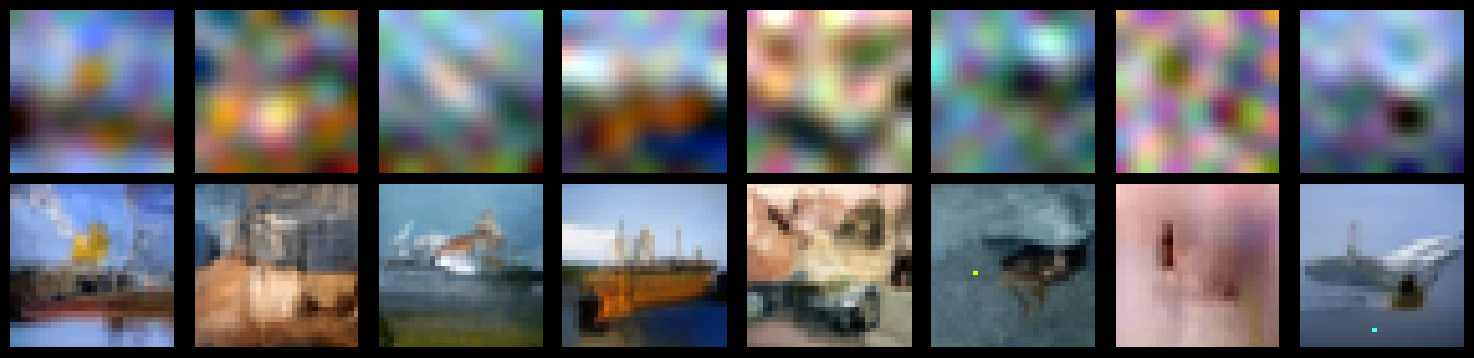
\includegraphics[width=0.85\textwidth]{pics/5_dvp/cifar10_dct_prior_samples.pdf} \\
%         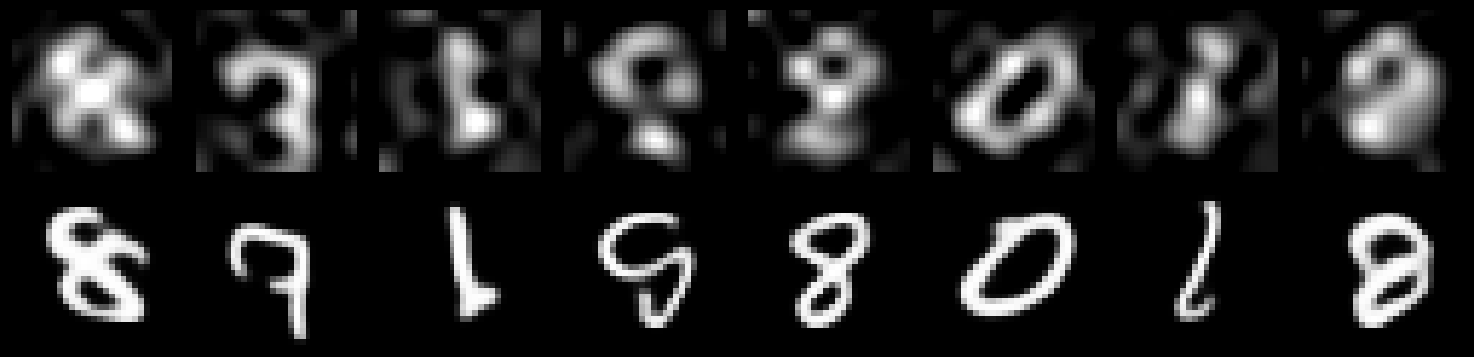
\includegraphics[width=0.85\textwidth]{pics/5_dvp/mnist_dct_prior_samples.pdf} \\
%         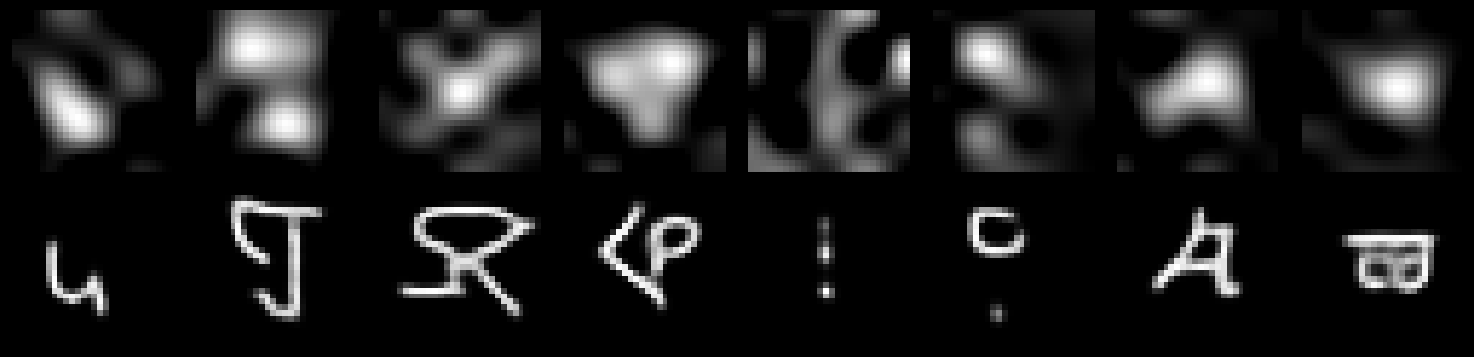
\includegraphics[width=0.85\textwidth]{pics/5_dvp/omniglot_dct_prior_samples.pdf} \\
%     \end{tabular}
%     \caption{Unconditional samples from the Diffusion-based VampPrior (top) and corresponding samples from the DVP-VAE (bottom).}
%     \vskip -5pt
%     \label{fig:dct_samples}
% \end{figure}
% \end{minipage}\hfill
% \begin{minipage}[t]{.65\linewidth}
% \begin{figure}[H]
%     \begin{tabular}{cc}
%         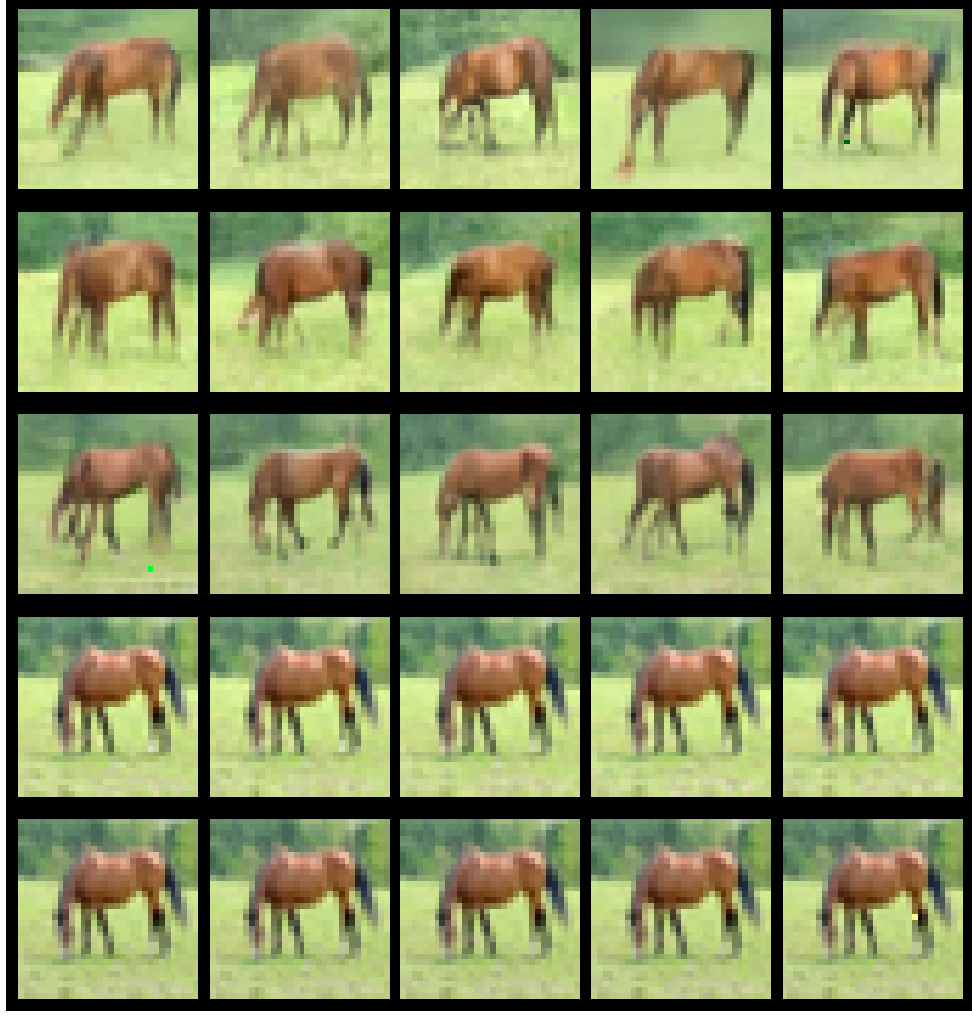
\includegraphics[width=0.43\textwidth]{pics/5_dvp/cifar10_generative_rec_6.pdf} &
%         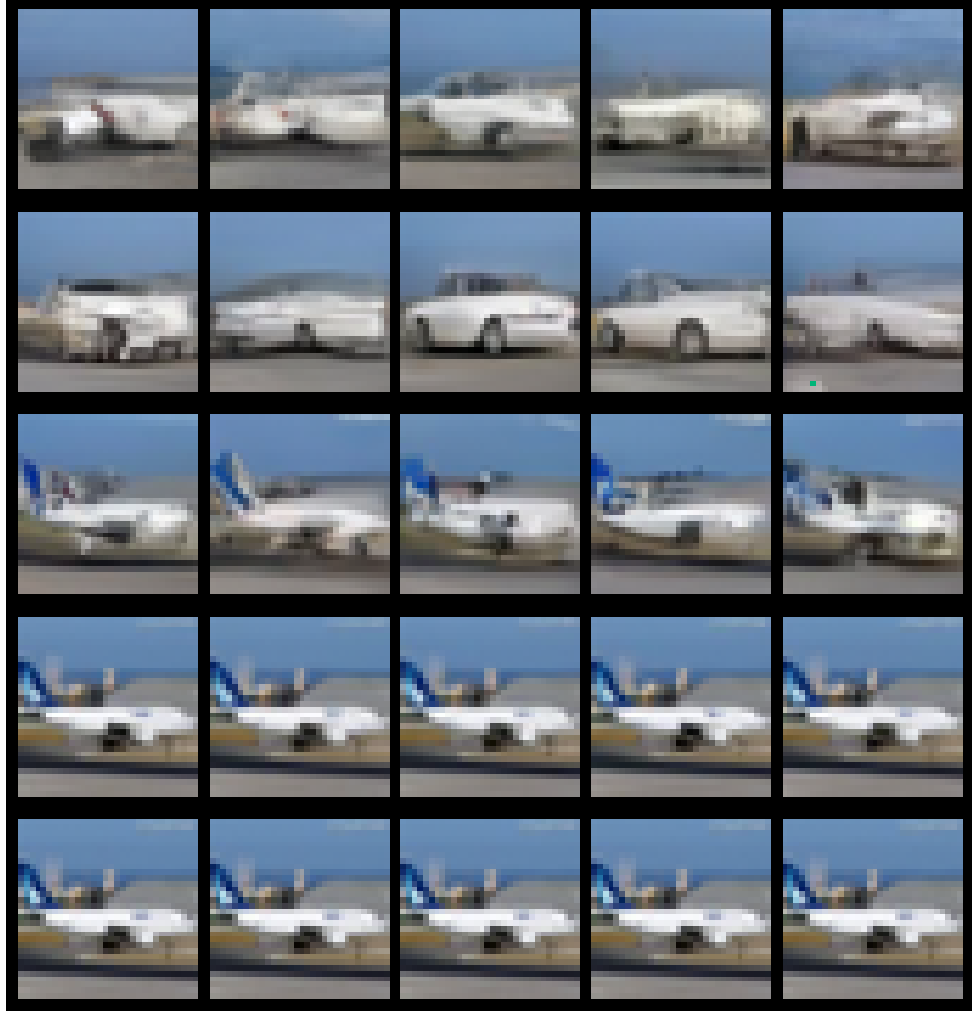
\includegraphics[width=0.43\textwidth]{pics/5_dvp/cifar10_generative_rec_9.pdf} \\ 
%     \end{tabular}
%     \caption{\textit{Generative reconstruction}s. The top row is using a pseudoinput sampled from $r(\rvu|\rvx)$ \textbf{only}.}
%     \vskip -5pt
%     \label{fig:generative_recon}
% \end{figure}
% \end{minipage}\hfill
% \end{table}



%%%%%%%%%%%%%%%%% POSTERIOR COLLAPSE %%%%%%%%%%%%%%%%%

%----SECTION----
\subsection{Ablation Studies}\label{sect:ablation}


\paragraph{Training stability and convergence}

% We employ severla changes in the architecture, which were made to improve training stability. 

In all of our experiments, we did not observe many training instabilities. 
Unlike many contemporary VAEs, we did not use gradient skipping \citep{Child2020-ze}, spectral normalization \citep{vahdat2020nvae}, or softmax parameterization of variances \citep{hazami2022efficientvdvae}. 
We use the Adamax version of the Adam optimizer \citep{kingma2015adam} following \citet{hazami2022efficientvdvae}, as it demonstrated much better convergence for the model with a mixture of discretized logistic likelihood. 

First, we observe a consistent performance improvement as we increase the model size and the number of stochastic layers. 
In Table~\ref{tab:increase_num_layers}, we report test performance and the percentage of active units (see Section~\ref{subsec:active_units} for details) for models of different stochastic depths trained on the CIFAR10 dataset. 
We train each model for 500 epochs, which corresponds to less than 200k training iterations. 
Additionally, we report gradient norms and training and validation losses for all four models in Appendix~\ref{appx:depth_experiment}. 


To demonstrate the advantage of the proposed architecture, we compare our model to a closest deep hierarchical VAE architecture: Very Deep VAE. For this experiment, we chose hyperparameters closest to Table 4 in \cite{Child2020-ze} (CIFAR-10). That is, our model has 45 stochastic layers and a comparable number of trainable parameters. Furthermore, following \cite{Child2020-ze}, we train this model with a batch size of 32, a gradient clipping threshold of 200, and an EMA rate of 0.9998. 
% We trained a model with the same number of stochastic layers (45) and similar number of parameters. 
% We used the same batch size (32) and gradient clipping (200). 
However, in DVP-VAE, we were able to eliminate gradient skipping and gradient smoothing. 
We report the difference in key hyperparameters and test performance in Table \ref{tab:ablation_stability}. We also add a comparison with Efficient-VDVAE (see Table 3 in \cite{hazami2022efficientvdvae}).
We observe that DVP-VAE achieves comparable performance within much fewer training iterations than both VDVAE implementations. 


\begin{table*}[t]
\begin{minipage}[t]{.3\linewidth}
    % \vskip -10pt   
    \centering
    \captionof{table}{Test performance for the model trained for 500 epochs (or approximately 200k training iterations) on CIFAR10.}    \label{tab:increase_num_layers}
    \begin{tabular}{ll|cc}
        \toprule
         \textsc{L} & \textsc{Size} & \textsc{BPD}$\leq$ $\downarrow$ & \textsc{AU} $\uparrow$\\
        \midrule
        20 & 24M & 2.99 & 94\%\\
        28 & 32M & 2.94 & 93\% \\
        36 & 40M & 2.89 & 98\%\\
        44 & 48M & 2.84 & 97\%\\
        \bottomrule
    \end{tabular}
    \vskip -25pt   
\end{minipage}\hfill
\begin{minipage}[t]{.67\linewidth}
    % \vskip -10pt   
    \centering
    \captionof{table}{Training settings for the model trained on CIFAR-10 compared to two VDVAE implementations. 
    % Both models have 45 stochastic layers and are trained with batch size 32.
    }
    \vskip -5pt   
    \label{tab:ablation_stability}
    \small{
    \begin{tabular}{l|ccc}
        \toprule
         & \small{\textsc{VDVAE}} & \small{\textsc{Efficient-VDVAE}} &\small{\textsc{DVP-VAE}} \\
         & \footnotesize{\citep{Child2020-ze}} & \footnotesize{\citep{hazami2022efficientvdvae}}&\footnotesize{(ours)}\\
        \midrule
        \textsc{L} & 45 & 47 & 45 \\
        \textsc{Size} & 39M & 57M & 38M \\
        % Batch size & 32 & 16 & 32\\
        \textsc{Optimizer} & \textsc{AdamW} & \textsc{Adamax} & \textsc{Adamax}\\
        \textsc{Learning rate} & 2e-4 & 1e-3 & 1e-3\\
        % \textsc{Weight decay} & 1e-2 & &1e-6\\
        \textsc{Grad. smoothing} & -- & Yes & --\\
        \textsc{Grad. skip} & 400 & 800 & --\\
        % Grad. clip & 200 & 200\\
        % EMA rate & 0.9998 & 0.9998\\
        \textsc{Training iter.} & 1.1M & 0.8M &\textbf{0.4M} \\
        % \small{GPUs}  & 2$\times$V100 & 1$\times$A100\\
        % \small{Training time} & 6 days & \ak{$\sim$ 5 days}\\
        \midrule
        \textsc{Test BPD} & 2.87 & 2.87 &2.86 \\
        \bottomrule
    \end{tabular}
    }
    \vskip -30pt   
\end{minipage}
\end{table*}


\paragraph{Latent Aggregation Increases Latent Space Utilization}\label{subsec:active_units}

Next, we test the claim that latent variable aggregation discussed in Sec.~\ref{subsec:latent_aggr} improves latent space utilization. We use Active Units (AU) metric~\citep{burda2015importance}, which can be calculated for a given threshold $\delta$ as follows:
\begin{align}\label{eq:active_units}
\text{AU} &= \frac{\sum_{l=1}^L \sum_{i=1}^{M_l}  \left[\text{A}_{l, i} > \delta \right] }{\sum_{l=1}^L M_l }, \\
    \text{where } \text{A}_{l} &= \text{Var}_{q^{\text{test}}(\rvx)} \E_{q_{\phi}(\rvz_{l+1:L}|\rvx)} \E_{q_{\phi}(\rvz_l | \rvz_{l+1:L}, \rvx)}\left[\rvz_l\right].
\end{align}
Here $M_{l}$ is the dimensionality of the stochastic layer $l$, $\left[ B \right]$ is the Iverson bracket, which equals $1$ if $B$ is true and $0$ otherwise, and $\text{Var}$ stands for variance.
Following \citet{burda2015importance}, we use the threshold $\delta = 0.01$. The higher the share of active units, the more efficient the model is in utilizing its latent space. 

We report results in Table~\ref{tab:ablation_active_units} and observe that the model with latent aggregation always attains more than 90\% of active units. Furthermore, latent aggregation considerably improves the utilization of the latent space if we compare it with exactly the same model but with the conditional likelihood parameterized using deterministic feature from the TopDown path (see Eq.~\ref{eq:cond_like_vdvae}).
\begin{table}[t]
\begin{minipage}[t]{.51\linewidth}
   \centering
       \captionof{table}{Active Units for the DCT-VAE with and without latent aggregation. 
       }
    \label{tab:ablation_active_units}
    \small{
    \begin{tabular}{ccc|c}
        \toprule
             \footnotesize{\textsc{Latent Aggr.}}& \footnotesize{\textsc{Size}} &
             \footnotesize{\textsc{L}} & \footnotesize{\textsc{AU}} $\uparrow$  \\
            \midrule
                \multicolumn{3}{c}{\footnotesize{\textsc{MNIST}}} \\
            \midrule
          \ding{55}   & 0.7M & 8 & 33.2\%\\
          $\checkmark$& 0.7M & 8 & 91.5\%\\
        \midrule
                \multicolumn{3}{c}{\footnotesize{\textsc{OMNIGLOT}}} \\
            \midrule
         \ding{55}    & 1.3M & 8 & 71.3\%\\
         $\checkmark$ & 1.3M & 8 & 93.4\%\\
         \midrule
                \multicolumn{3}{c}{\footnotesize{\textsc{CIFAR10}}} \\
            \midrule
         $\checkmark$    &  19.5M & 28 & 98\%\\
        \bottomrule
    \end{tabular}
    }
\end{minipage}\hfill
\begin{minipage}[t]{0.50\linewidth}
\centering
      \captionof{table}{Test NLL for the model with and without pseudoinputs. Averaged over 4 random seeds, standard deviation in parenthesis.}
    % \vskip 5pt
    \label{tab:ablation_nll}
    \small{
    \begin{tabular}{cc|c}
        \toprule
              \footnotesize{\textsc{Pseudoinputs}} & \footnotesize{\textsc{Size}} & \footnotesize{\textsc{NLL}}$\downarrow$  \\
            \midrule
                \multicolumn{3}{c}{\footnotesize{\textsc{MNIST}}} \\
            \midrule
        \ding{55}    & \footnotesize{0.6M} & 78.85 \footnotesize{(0.24)} \\
        $\checkmark$ & \footnotesize{0.7M} & 77.10  \footnotesize{(0.05)}\\ 
        \midrule
        \multicolumn{3}{c}{\footnotesize{\textsc{OMNIGLOT}}} \\
        \midrule
         \ding{55} & \footnotesize{1.1M} & 89.52 \footnotesize{(0.23)}\\
     $\checkmark$  & \footnotesize{1.3M} & 89.07 \footnotesize{(0.10)}\\
        \bottomrule
    \end{tabular}
    }
\end{minipage}\hfill
\end{table}


\begin{figure}[t]
    \begin{tabular}{cc}
        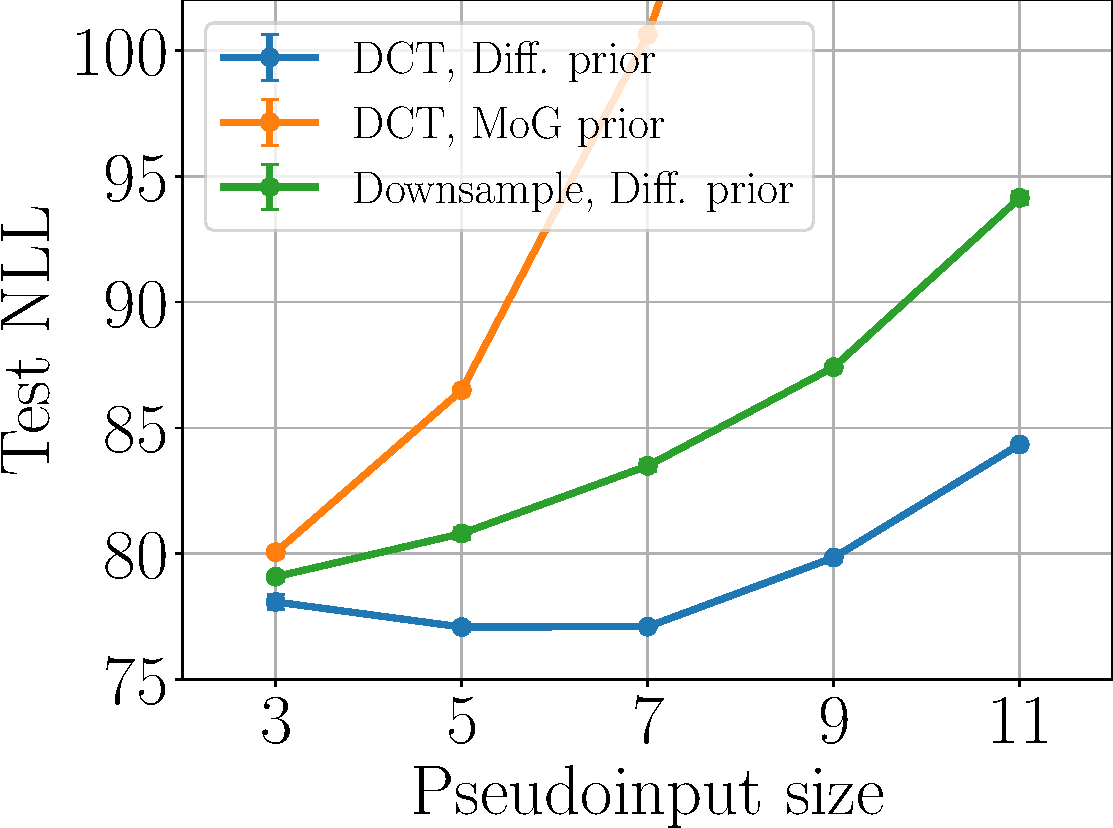
\includegraphics[width=0.43\linewidth]{pics/5_dvp/mnist_ctx_ablaions_line.pdf} &
        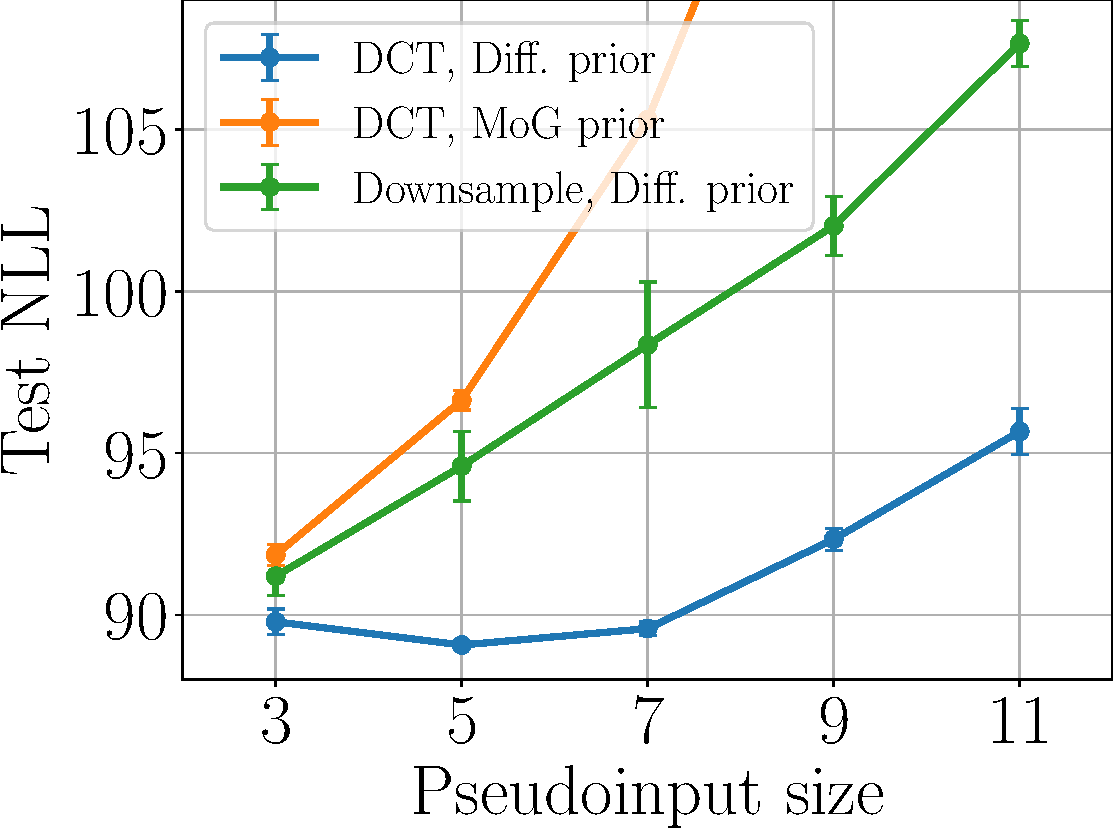
\includegraphics[width=0.43\linewidth]{pics/5_dvp/omniglot_ctx_ablaions_line.pdf} \\
        (a) MNIST &
        (b) OMNIGLOT \\
    \end{tabular}
    \vskip -3pt
    \caption{Ablation study of for the pseudoinputs type (DCT and Downsampled image), pseudoinputs prior (Diffusion model and Mixture of Gaussians) and pseudoinputs size (ranging from $3\times 3$ to $11\times 11$). Each configuration is trained with four different random seeds.}
    \label{fig:mnist_ctx_ablations}
\end{figure}
\begin{figure}[t]
    \begin{tabular}{cc}
        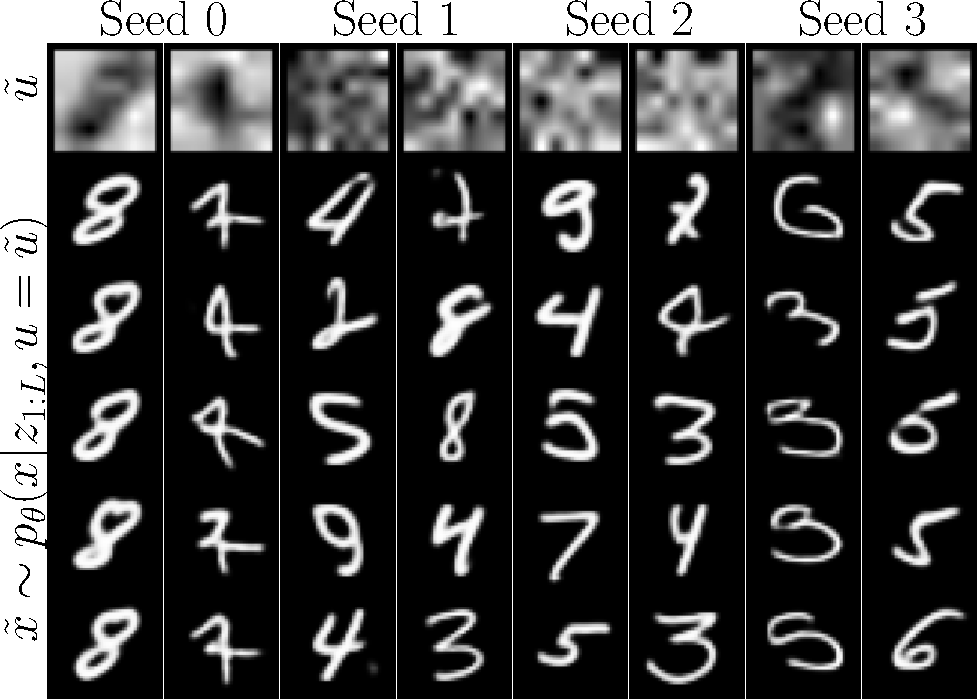
\includegraphics[width=0.43\textwidth]{pics/5_dvp/mnist_linear_prior_samples.pdf} &
        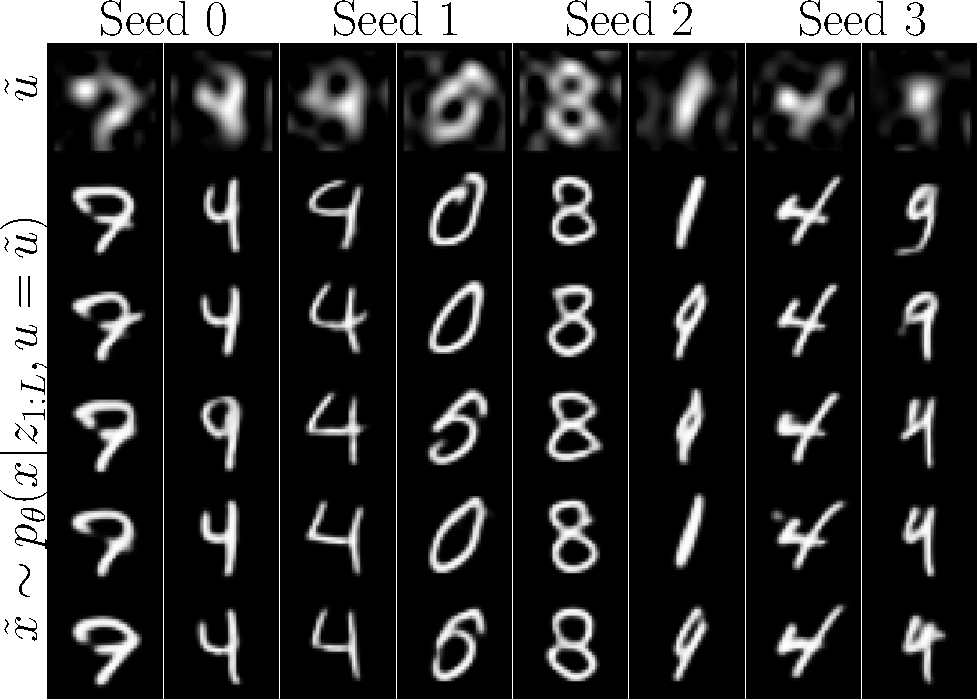
\includegraphics[width=0.43\textwidth]{pics/5_dvp/mnist_dct_prior_samples_seed.pdf} \\ \\
        (a) Learnable pseudoinputs &
        (b) DCT pseudoinputs \\
    \end{tabular}
    \caption{Samples from the pseudoinputs prior $\Tilde{\rvu} \sim \hat{r}(\rvu)$ (top row) and corresponding samples from the model $\Tilde{\rvx} \sim p_{\theta}(\rvx|\rvz_{1:L}, \rvu=\Tilde{\rvu})$ (other rows). Columns corresponds to models trained with different random seeds.}
    \label{fig:linear_context_sampels}
\end{figure}


\paragraph{Amortized VampPrior Improves BPD}

Further, we test how the proposed amortized VampPrior improves model performance as measured by the negative log-likelihood. We report results in Table~\ref{tab:ablation_nll} and observe that DVP-VAE always has a better NLL metric compared to the deep hierarchical VAE with the same architecture and number of stochastic layers.
Due to additional diffusion-based prior over pseudoinputs, DVP-VAE has slightly more trainable parameters. However, because of the small spatial dimensionality of the pseudoinputs, we were able to keep the size of the two models comparable. 

\paragraph{Pseudoinputs type, size and prior}
We conduct an extensive ablation study regarding pseudoinputs. First, we train VAE with two types of pseudoinputs: DCT and Downsampled images. Moreover, we vary the spatial dimensions of the pseudoinputs between $3\times 3$ and $11\times 11$. We expect that a smaller pseudoinputs size will be an easier task for the prior $\hat{r}(\rvu)$, but will constitute a poorer approximation of an optimal prior. The larger pseudoinput size, on the other hand, results in a better optimal prior approximation since more information about the datapoint $\rvx$ is preserved. However, it becomes harder for the prior to achieve good results since we keep the prior model size fixed.
In Figure~\ref{fig:mnist_ctx_ablations} we observe that the DCT-based transformation performs consistently better across various sizes and datasets. 

\paragraph{Trainable Pseudoinputs}
In the VampPrior, the optimal prior is approximated using learnable pseudoinputs. In this work, on the other hand, we propose to use fixed linear transformation instead. To further verify whether a fixed transformation like DCT is reasonable, we checked a learnable linear transformation. We present in Figure~\ref{fig:linear_context_sampels} that the learnable linear transformation of the input exhibits unstable behavior in terms of the \textbf{quality} of learned pseudoinput. The top row of Figure~\ref{fig:linear_context_sampels}(a) shows samples from the trained prior and the corresponding samples from the decoder. 
We observe that only one out of four models with learnable pseudoinputs was able to learn a visually meaningful representation of the data (seed 0), which also resulted in very high variance of the results (rows below). For other models (e.g., Seed 1 and Seed 2), the same pseudoinput sample corresponds to completely different datapoints.

This lack of consistency motivates us to use a non-trainable transformation for obtaining pseudoinputs. In Figure~\ref{fig:linear_context_sampels}~(b), we show the expected behavior of sampling semantically meaningful pseudoinputs that is consistent across random seeds.
% Each row corresponds to the model trained with different random seeds.


\begin{wraptable}{l}{0.49\textwidth}
\small{
% \resizebox{\linewidth}{!}{
    \vskip -15pt   
    \centering
    \caption{Wall-clock time, memory consumption and sampling time for DVP and VampPrior.}
    \label{tab:vamp_scalability}
        \begin{tabular}{ll|ccc|cc}
            \toprule
            % \multirow{2}{*}{\textsc{Model}} 
            & \multirow{2}{*}{\small{\textsc{K}}} &
             \textsc{Train} & \textsc{GPU} & \textsc{Size} & \textsc{Sample} \\
             &  &\textsc{time}  & \textsc{mem.} &   &  \textsc{time}
             \\ \midrule
                && \multicolumn{3}{c}{\footnotesize{\textsc{MNIST (32 channels)}}} \\
            \midrule
            DVP &  N/A  & 45s & 3Gb & 0.7M & 2.2 \\
            \multirow{2}{*}{Vamp}
                & 500   & 45s & 4Gb & 1.0M & 0.2\\
                & 1000  & 60s &  6Gb & 1.4M & 0.3\\
                \midrule
            && \multicolumn{3}{c}{\footnotesize{\textsc{MNIST (64 channels)}}} \\
            \midrule
            DVP &  N/A  & 50s & 4Gb & 2.4M & 2.3\\
            \multirow{2}{*}{Vamp}& 500   & 65s &  7Gb & 2.7M & 0.5\\
                & 1000  & 90s &  10Gb & 3.1M & 0.8\\
            \midrule
            \midrule
                && \multicolumn{3}{c}{\footnotesize{\textsc{CIFAR10}}} \\
            \midrule
            DVP &  N/A  & 370s & 12Gb  & 19.5M & 4.0\\
            \multirow{3}{*}{Vamp}& 500   & 430s  & 29Gb  & 20.5M & 1.5\\
                & 750   & 500s & 38Gb  & 21.3M & 1.8\\
                & 1000  & OOM  & >40Gb & 22.1M & ---\\
            \bottomrule
        \end{tabular}% % \end{varwidth}%\hfill 
% \end{minipage}
\vskip -5pt
}
\end{wraptable} 

\paragraph{Scalability}
Here, we study how DVP-VAE scales as we increase model size and input size in comparison with VampPrior.
% how the wall-clock training time and the memory requirements of the DVP-VAE compares to the original VampPrior. 
For this, we implement VampPrior as proposed by \cite{tomczak2018vae}, where the top latent variable is trained with the VampPrior and the other layers with the conditional Gaussian (see Eq.~\ref{eq:hierarchical_vamp}).
 We use the same architecture as in main experiments for MNIST (32 channels) and CIFAR10 (see Table~\ref{tab:setup}). Additionally, we train model with doubled number of channels on MNIST (64 channels).

In Table \ref{tab:vamp_scalability}, we report the training time (second per epoch), GPU memory utilization and total number of trainable parameters. 
We observe that VampPrior almost always utilizes significantly more memory and requires longer training time. The difference is less visible on a small model and small input size (MNIST, 32 channels). However, as we double number of channels, both training time and memory utilization for VampPrior grows much faster. As a result, for a bigger input size (CIFAR10 dataset) a model with more than 750 pseudoinputs does not fit into a single A100 GPU. For 500 pseudoinputs, memory utilization is already 2.5 times higher for VampPrior compared to DVP-VAE.
% Furthermore, the wall-clock training time for the original VampPrior is larger than for our approach, and training gets slower as we increase the number of pseudoinputs.


% \begin{minipage}[t]{.6\linewidth}



% Table 1. MNIST. Experiments on a single RTX 2080 GPU
% |       |      | Training      |   Inference   | GPU memory (Gb) | # Params |
% |       |      | (1 epoch, s)  | (1 image, ms) |                 |          |
% |-------|------|---------------|---------------|-----------------|----------|
% | DVP   |      |    45         |   1.6         |      3 Gb       | 0.7 M    |
% | Vamp  | 500  |    45         |   0.3         |      4 Gb       | 1.0 M    |
% |       | 1000 |    60         |   0.4         |      6 Gb       | 1.4 M    |
% |       | 1500 |    70         |   0.5         |      8 Gb       | 1.8 M    |

% Table 2. Cifar10. Experiments on a single A100 GPU
% |       |      | Training      |   Inference   | GPU memory (Gb) | # Params  |
% |       |      | (1 epoch, s)  | (1 image, ms) |                 |           |
% |-------|------|---------------|---------------|-----------------|-----------|
% | DVP   |      |     370       |     5.4       |        12 Gb    |  19.5 M   |
% | Vamp  | 500  |     430       |     1.4       |        29 Gb    |  20.5 M   |
% |       | 750  |     500       |     1.7       |        38 Gb    |  21.3 M   |
% |       | 1000 |    – (OOM)    |   — (OOM)     |        >40 Gb   |  22.1 M   |

